% !Mode:: "TeX:UTF-8"
\documentclass{article}
\usepackage{graphicx}
\usepackage{CJK}
\usepackage{amsmath}
\usepackage{tabularx}
\usepackage{anysize}
\usepackage{graphicx}
\usepackage{subfigure}
\marginsize{2cm}{2cm}{-1cm}{2cm}

\begin{document}
\begin{CJK}{UTF8}{gkai} % gbsn: 宋体简化字；gkai 楷体简化字; bsmi 繁体宋书；bkai 繁体楷书

\renewcommand{\abstractname}{摘 \qquad 要}
\renewcommand{\contentsname}{\center 目\qquad\qquad录}
\renewcommand{\listfigurename}{图 \quad 示 \quad 目 \quad 录}
\renewcommand{\listtablename}{表 \quad 格 \quad 目 \quad 录}
\renewcommand{\appendixname}{附录}
\renewcommand{\refname}{\center 参 \quad 考 \quad 文 \quad 献}
%\renewcommand{\bibname}{专著}
\renewcommand{\indexname}{\center 索 \qquad 引}
\renewcommand{\figurename}{图}
\renewcommand{\tablename}{表}
%\renewcommand{\pagename}{页}

\title{HW1-GitPages}
\author{软件学院-李书昂（2014013431）}
\date{\today}
\maketitle

\section{作业要求}
	\subsection{基础部分}
		\begin{enumerate}
		\item 个人主页包括一个或多个页面，含个人介绍、照片以及联系方式。
		\item 个人主页中包含Web前端课程展示区。
		\item 个人主页中发布第一篇个人日志。
		\item 个人主页使用Github Pages发布。
		\item 个人主页需协调美观，支持Chrome、Safari、Firefox等主流浏览器。
		\end{enumerate}
	\subsection{提高要求}
		\begin{enumerate}
		\item 使用Grunt或Gulp编写构建脚本，实现html、css压缩功能。
		\item 移动端的页面适应。
		\end{enumerate}

\section{网页设计与实现}
	\subsection{网页结构}
	该主页结构主要分为：head,body(header,aboutme,work,blog,quote,footer)。
	\subsection{网页特色}
	\begin{enumerate}
	\item 其中header实现导航栏，在css中设置scrollup，单击时，可使网页下拉到特定位置，非常人性化。
	\item 鼠标悬浮到图标上时，图标呈现高亮状态。网页中有blog区,以及web课程作业展示区，skill展示区。
	\item 由于宋体等字体太丑，于是通过网上找了各种好看的字体css加入到了我的网页。
	\item 实现了移动端，ipad端的网页自适应。
		\begin{figure}
			\centering
			\subfigure[Html in iphone6]{
				\label{Fig.sub.1}
				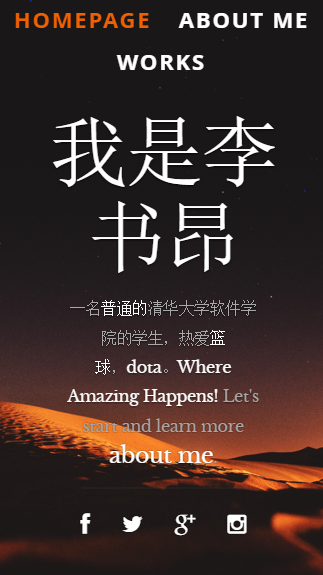
\includegraphics[width=1.5in,height=1.7in]{1.png}
				}
			\subfigure[Html in ipad]{
				\label{Fig.sub.2}
				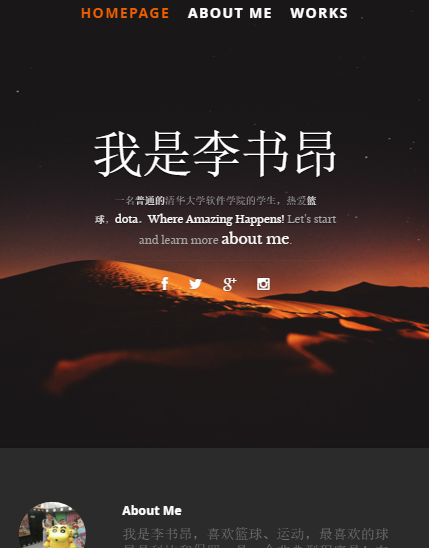
\includegraphics[width=1.5in,height=1.7in]{2.png}
				}
			\label{Fig.lable}
		\end{figure}
	\end{enumerate}
\end{CJK}
\end{document}